\documentclass[11pt]{beamer}
\usetheme{Rochester}
\usepackage[utf8]{inputenc}
\usepackage{amsmath}
\usepackage{amsfonts}
\usepackage{amssymb}
\usepackage{graphicx}
%\author{}
%\title{}
%\setbeamercovered{transparent} 
%\setbeamertemplate{navigation symbols}{} 
%\logo{} 
%\institute{} 
%\date{} 
%\subject{} 
\begin{document}

\begin{frame}
\title{Computational Astrophysics}
\author{E. Larrañaga}
\institute{Observatorio Astronómico Nacional\\
Universidad Nacional de Colombia}
\titlepage
\end{frame}

\begin{frame}{Outline}
\tableofcontents
\end{frame}

\section{Linear Advection Equation}
\begin{frame}[fragile]{Linear Advection Equation}
The linear advection equation is 
\begin{equation}
\label{eq:advect}
\partial_t u + v \partial_x u = 0
\end{equation}
where $u(t,x)$ is some scalar quantity and $v$ is the constant velocity at
which it is advected ($v > 0$ advects to the right).\\ 

The solution to
this equation is to simply take the initial data, $u(t=0,x)$,
and displace it to the right at a speed $v$.  The shape of the initial
data is preserved in the advection. 
\end{frame}

\begin{frame}[fragile]{Linear Advection Equation}
 Many hyperbolic systems of PDEs,
e.g.\ the equations of hydrodynamics, can be written in a form that
looks like a system of (nonlinear) advection equations, so the
advection equation provides important insight into the methods used
for these systems.
\end{frame}

\begin{frame}[fragile]{Linear Advection Equation}
Direct substitution shows that $u(x - vt)$ is a solution to
advection equation for any choice of u.\\
\bigskip 

This means that
the solution is constant along the lines $x = v t$
(the curves along which the solution is constant are called the
characteristics).
\end{frame}

\begin{frame}[fragile]{Linear Advection Equation}
\begin{center}
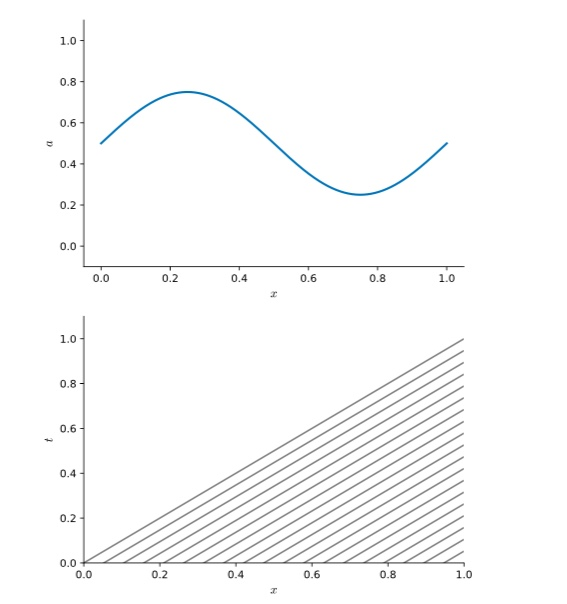
\includegraphics[scale=0.3]{advectioncharact}
\end{center}
\end{frame}


\section{Non-linear Hyperbolic Differential Equations. Burguer's Equation }
\begin{frame}[fragile]{Non-linear Hyperbolic Differential Equations. Burguer's Equation }
Burgers' equation is the simplest {\em nonlinear} hyperbolic
equation,
\begin{equation}
\partial_t u + u \partial_x u = 0.
\end{equation}
It is almost identical to the advection equation treated before, but this time the wave speed is 
NOT a constant $v$ but is
given by the field $u$ itself. 
\bigskip

Hence, $u$ is both the quantity being advected and the speed at which
it is moving.
\end{frame}

\begin{frame}[fragile]{Non-linear Hyperbolic Differential Equations. Burguer's Equation }
For the linear advection equation, the solution was constant along lines $x = vt + x_0$, which are
parallel, since $v$ is spatially constant.  
\bigskip

For Burgers' equation,
this is no longer the case, and the characteristic lines are now
given by $\frac{dx}{dt} = u$, with $x(0) = x_0$.  \\

Since $u = u(t)$, we cannot integrate this directly.
\end{frame}
  
\begin{frame}[fragile]{Burguer's Equation. Shocks}
 If we take $u_0 = u(t=0)$, then we can look at how the characteristic
behave over a small time interval (before $u(x,t)$ changes
significantly).\\
Next figure shows the behavior for
an initial velocity with sinusoidal profile.  
\end{frame}

\begin{frame}[fragile]{Burguer's Equation. Shocks}
\begin{center}
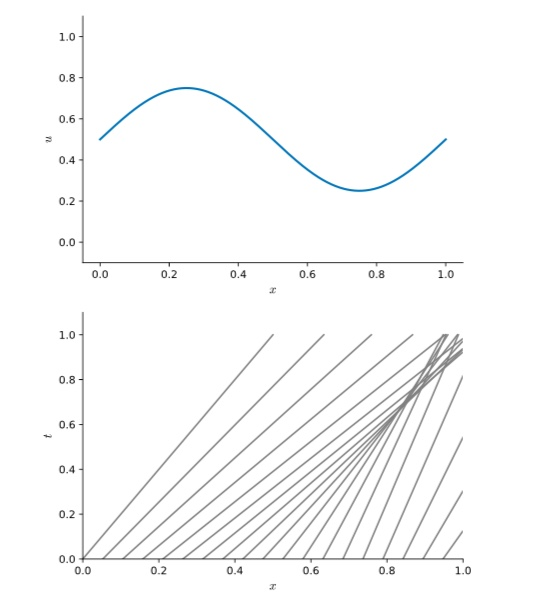
\includegraphics[scale=0.3]{burguerscharact}
\end{center}
\end{frame}

\begin{frame}[fragile]{Burguer's Equation. Shocks}
We see that after a
short period of time, the characteristics intersect.  At the point,
$(x_s, t_s)$ where they intersect, there is no way to trace backwards
along the characteristics to find a unique initial state.  \\
\bigskip

This
merging of the characteristics in the $x$-$t$ plane is a {\em shock}, and
represents just one way that nonlinear problems can differ from linear
ones.
\end{frame}

\begin{frame}[fragile]{Burguer's Equation. Shocks}
\begin{center}
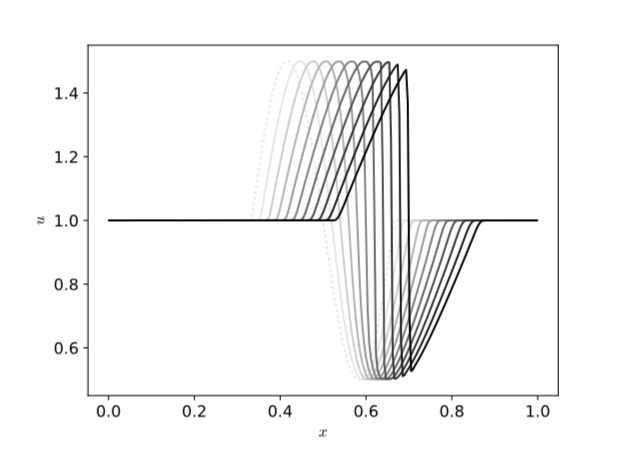
\includegraphics[scale=0.3]{burguershock}
\end{center}
\end{frame}

\begin{frame}[fragile]{Burguer's Equation. Rarefaction}
Another type of wave not present in a linear system is a {\em
  rarefaction}.  Next figure shows initial
conditions of slower velocity to the left of faster velocity. 
\bigskip

 We see
that the characteristics diverge in this case, and we will be left
with having to fill in the solution inbetween as some intermediate
state.
\end{frame}

\begin{frame}[fragile]{Burguer's Equation. Rarefaction}
\begin{center}
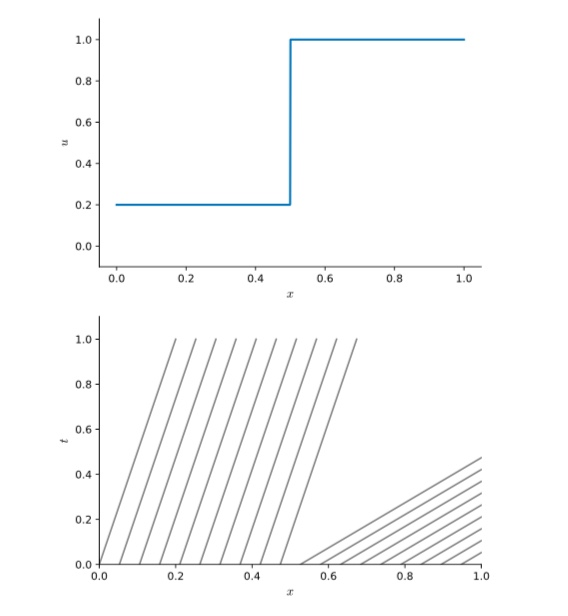
\includegraphics[scale=0.3]{burguerscharact2}
\end{center}
\end{frame}

\begin{frame}[fragile]{Burguer's Equation. Rarefaction}
\begin{center}
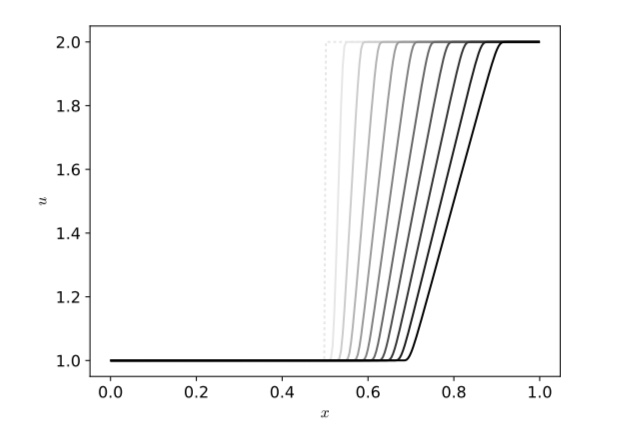
\includegraphics[scale=0.3]{burguersrarefaction}
\end{center}
\end{frame}

\section{Matrix Method}
\begin{frame}[fragile]{Matrix Method}
In the matrix method, we discretize Poisson Equation
with centered differences. Then, for an interior (non-boundary) grid point $i$ we have
\begin{equation}
\begin{aligned}
\frac{\partial \Phi }{\partial r} \bigg|_i &\approx \frac{1}{2\Delta r} \left(\Phi_{i+1} - \Phi_{i-1}\right)\,\,,\\
\frac{\partial^2 \Phi }{\partial r^2}  \bigg|_i &\approx \frac{1}{(\Delta r)^2} \left(\Phi_{i+1} - 2 \Phi_i + \Phi_{i-1} \right)\,\,.
\end{aligned}
\end{equation}
Then, Poisson equation is
\begin{equation}
\begin{aligned}
\frac{1}{r_i} \frac{\left(\Phi_{i+1} - \Phi_{i-1}\right)}{\Delta r}  + \frac{\left(\Phi_{i+1} - 2 \Phi_i + \Phi_{i-1} \right)}{(\Delta r)^2}  &= 4\pi G \rho_i\,\,.
\end{aligned}
\end{equation}
\end{frame}

\begin{frame}[fragile]{Matrix Method}
\textbf{Inner boundary condition:}\\
Because of the $1/r$ term in the Laplacian, it is clear that the behavior 
 at $r=0$ must be regularized. \\
 \bigskip
 
 It is possible to use an expansion or we can
stagger the grid so that there is no point exactly at $r=0$, for example 
by moving the entire grid over by $0.5 \Delta r$.  \\
\end{frame}

\begin{frame}[fragile]{Matrix Method}
\textbf{Inner boundary condition:}\\
At the inner boundary, we have the condition $\frac{\partial \Phi}{ \partial r} = 0$, so we assume
\begin{equation}
\Phi_{-1} = \Phi_{0}\,\,.
\end{equation}
\end{frame}

\begin{frame}[fragile]{Matrix Method}
Hence, Poisson equation can be written as linear system
\begin{equation}
J \mathbf{\Phi} = \mathbf{b}\,\,,
\label{eq:pde_poisson2}
\end{equation}
where $\Phi$ = $(\Phi_0, \cdots , \Phi_{n-1})^T$ (for a grid with $n$
points labeled $0$ to $n-1$) and  $\mathbf{b} = 4\pi G
(\rho_0, \cdots , \rho_{n-1})^T$. 
\end{frame}

\begin{frame}[fragile]{Matrix Method}
The matrix $J$ has tri-diagonal form and can be explicitely given as:
\begin{itemize}
\item[(a)] $i=j=0$:
\begin{equation}
J_{00} = - \frac{1}{(\Delta r)^2} - \frac{1}{r_0 \Delta r}\,\,,
\end{equation}
\item[(b)] $i=j$:
\begin{equation}
J_{ij} = \frac{-2}{(\Delta r)^2}\,\,,
\end{equation}
\item[(c)] $i+1=j$:
\begin{equation}
J_{ij} = \frac{1}{(\Delta r)^2} + \frac{1}{r_i \Delta r}\,\,,
\end{equation}
\item[(d)] $i-1=j$:
\begin{equation}
J_{ij} = \frac{1}{(\Delta r)^2} - \frac{1}{r_i \Delta r}\,\,.
\end{equation}
\end{itemize}
\end{frame}

\begin{frame}[fragile]{Matrix Method}
After finding the solution to the linear system, it is neccesary to correct for the analytic outer boundary
value 
\begin{equation}
\Phi(R_\text{surface}) = - \frac{G M}{R_\text{surface}}.
\end{equation}
\end{frame}


\begin{frame}[fragile]{Next Class}
Poisson Equation
\end{frame}

\end{document}
